\chapter{Προσαρμογή Γραμμικού Μοντέλου}
\label{ch:step2}
\thispagestyle{fancy}

Με βάση τα συμπερασμάτα που εξήχθησαν από την ανάλυση στο πρώτο βήμα, το γραμμικό μοντέλο που θα προσαρμόσουμε στη χρονοσειρά Α είναι \tl{ARIMA} με $d=1$, καθώς:
\begin{itemize}
    \item παίρνοντας τις πρώτες διαφορές (στη μετασχηματισμένη με τετραγωνικές ρίζες αρχική χρονοσειρά), η χρονοσειρά που προκύπτει φαίνεται στα διαγράμματα ιστορίας και αυτοσυσχέτισης να είναι στάσιμη (η τάση έχει απαλειφθεί) και επιπλέον δεν υπάρχει εξάρτηση της διασποράς από τη τάση
    \item δεν φαίνεται να υπάρχει εποχικότητα και άρα η χρήση ενός \tl{ARIMA} μοντέλου θα είναι ικανοποιητική. Συγκεκριμένα δοκιμάστηκε η εκτίμηση της εποχικότητας (με μέσους όρους στοιχείων της περιόδου) και οι ακολουθίες που βρέθηκαν για περιόδους 5, 6 και 16 ημερών (καθώς αυτές είναι μόνες στατιστικά σημαντικές τιμές του διαγράμματος αυτοσυσχέτισης - σχήμα \ref{fig:xa_autocorrelation}) είναι [0.082,-0.0672,0.021,0.039,-0.075], [0.011,-0.033,-0.017,0.020,-0.106,0.1250] και [0.087,0.224,-0.176,-0.104,0.092,0.214,-0.057,-0.130,0.058,\\ -0.095,0.020,0.046,-0.069,0.219,-0.254,-0.075] αντίστοιχα. Δεδομένου ότι το εύρος τιμών της αντίστοιχης χρονοσειράς είναι περίπου στο [-3, 3] αλλά και ότι οι τιμές της αυτοσυσχετίσεις για τις συγκεκριμένες υστερήσεις είναι οριακά πάνω από το όριο σημαντικότητας, μπορούμε με ασφάλεια να εξάγουμε το συμπέρασμα ότι δεν υπάρχει εποχικός όρος στη χρονοσειρά των πρώτων διαφορών των τετραγωνικών ριζών, δηλαδή στη στάσιμη χρονοσειρά που καταλήξαμε.
\end{itemize}

\section{Προσαρμογή \tl{ARIMA(p,d,q)}}

\subsection{Προσαρμογή \tl{ARIMA(p,1,q)} παίρνοντας τις πρώτες διαφορές}

Έτσι, συνεχίζοντας την ανάλυση από το τέλος του βήματος 1, μετά την εφαρμογή των πρώτων διαφορών στη χρονοσειρά των τετραγωνικών ριζών έχουμε υλοποιήσει το πρώτο στάδιο προσαρμογής ενός μοντέλου \tl{ARIMA(p,d,q)} που είναι η εφαρμογή διαφορών \tl{d}-οστής. Άρα εδώ θα είναι $d=1$ και η χρονοσειρά που καταλήγουμε είναι η $\{X_a(t)\}$.\\
Το δεύτερο στάδιο είναι η εύρεση των παραμέτρων του μοντέλου \tl{ARMA(p,q)}, κάτι που αναλύεται στην επόμενη υπο-ενότητα. 

\subsection{Προσαρμογή \tl{ARMA(p,q)} στη στάσιμη χρονοσειρά}

Οι παράμετροι \tl{p} και \tl{q} είναι \tl{hyperparameters} του μοντέλου και επομένως το πρώτο μας μέλημα είναι να βρούμε το βέλτιστο συνδυσμό των παραμέτρων αυτών ή τάξεων του μοντέλου. Προς το σκοπό αυτό θα κάνουμε \tl{grid search} για τιμές των τάξεων από 0 (απουσία του αντίστοιχου όρου) έως και 10.\par

Για την αξιολόγηση του κάθε συνδυασμού χρησιμοποιήθηκαν τα κριτήρια πληροφορίας \tl{Akaike (AIC)} και \tl{Forward Prediction Error (FPE)}, τα οποία ορίζονται ως εξής:
\begin{align}
AIC(p,q) = \ln{\left(s_z^2\right)} + \frac{2\times(p+q)}{n}
\label{eq:aic}
\end{align}
και
\begin{align}
FPE(p,q) = s_z^2 \times \frac{n + (p+q)}{n - (p+q)}
\label{eq:fpe}
\end{align}
όπου $n$ είναι ο αριθμός των δειγμάτων που χρησιμοποιήθηκαν για την εκτίμηση των ροπών (π.χ για τη δειγματική αυτοσυσχέτιση) και $s_z^2$ είναι η (δειγματική) διασπορά των σφαλμάτων ή υπολοίπων που προκύπτουν όταν συγκρίνουμε τις τιμές του προσαρμοεσμένου μοντέλου τάξης $(p,q)$ με τις πραγματικές τιμές της χρονοσειράς (ενν. τη χρονοσειρά $\{X_a(t)\}$ που προέκυψε ως οι πρώτες διαφορές της χρονοσειράς των τετραγωνικώ ριζών της αρχικής χρονοσειράς προβολών του βίντεο Α, $\{Y_a(t)\}$). \par

Παρακάτω παρατίθενται οι τιμές του \tl{AIC} για τους συνδυασμούς των παραμέτρων $(p,q)=(0...10)$, φυσικά με εξαίρεση το συνδυασμό $(p,q)=(0,0)$:

\begin{table}[H]
\resizebox{\textwidth}{!}{%
\centering
\begin{tabular}{ |c|c|c|c|c|c|c|c|c|c|c|c|c| }
\hline
\space&\multicolumn{12}{c|}{$p$} \\\hline
\multirow{11}{*}{$q$} & \space & 0 & \cellcolor[HTML]{EDEDED}1 & 2 & 3 & 4 & 5 & 6 & 7 & 8 & 9 & 10\\\cline{2-13}
& \cellcolor[HTML]{EDEDED} 0&\space& \cellcolor{lightgray} -0.465&-0.463&-0.462&-0.461&-0.460&-0.459&-0.459&-0.457&-0.458&-0.457\\\cline{2-13}
&1&-0.211&-0.463&-0.463&-0.462&-0.462&-0.461&-0.460&-0.458&-0.456&-0.457&-0.456\\\cline{2-13}
&2&-0.306&-0.462&-0.462&-0.465&-0.463&-0.461&-0.460&-0.457&-0.456&-0.459&-0.458\\\cline{2-13}
&3&-0.376&-0.461&-0.462&-0.463&-0.462&&-0.458&-0.459&-0.457&-0.458&-0.457\\\cline{2-13}
&4&-0.395&-0.46&-0.461&-0.462&&&-0.463&-0.460&-0.462&-0.457&-0.456\\\cline{2-13}
&5&-0.427&-0.460&-0.459&-0.460&-0.459&-0.461&-0.459&&-0.455&-0.455&-0.457\\\cline{2-13}
&6&-0.436&-0.459&-0.458&-0.459&-0.459&-0.460&&-0.463&-0.457&-0.458&-0.455\\\cline{2-13}
&7&-0.448&-0.458&-0.456&-0.457&-0.457&-0.457&-0.456&-0.457&-0.462&-0.454&-0.453\\\cline{2-13}
&8&-0.449&-0.458&-0.456&-0.459&-0.458&-0.456&-0.456&-0.457&-0.454&-0.462&-0.455\\\cline{2-13}
&9&-0.447&-0.456&-0.456&-0.455&-0.456&-0.456&-0.455&-0.455&-0.454&-0.452&-0.456\\\cline{2-13}
&10&-0.446&-0.456&-0.454&-0.454&-0.455&-0.454&-0.453&-0.459&-0.456&&-0.456\\\hline
\end{tabular}}
\caption{Αναζήτηση Πλέγματος με βάση τη μετρική \tl{AIC} για διάφορες τιμές των τάξεων $(p,q)$. Τα κενά κελιά σηματοδοτούν ότι για τον αντίστοιχο συνδυασμό τάξεων το προκύπτον \tl{ARMA} μοντέλο δεν ήταν στάσιμο, αντιστρέψιμο ή και τα δύο.}
\label{table:grid_search_aic}
\end{table}

από όπου φαίνεται πως η χαμηλότερη τιμή του \tl{AIC} επιτυγχανέται όταν προσαρμοζέται μοντέλο $ARMA(0,1)$ ή, ισοδύναμα, μοντέλο $MA(1)$. Ακολούθως δίνονται οι τιμές του \tl{FPE} για τους αντίστοιχους συνδυασμούς τιμών των \tl{p} και \tl{q}:

\begin{table}[H]
\resizebox{\textwidth}{!}{%
\centering
\begin{tabular}{ |c|c|c|c|c|c|c|c|c|c|c|c|c| }
\hline
\space&\multicolumn{12}{c|}{$p$} \\\hline
\multirow{11}{*}{$q$} & \space & 0 & \cellcolor[HTML]{EDEDED}1 & 2 & 3 & 4 & 5 & 6 & 7 & 8 & 9 & 10\\\cline{2-13}
& \cellcolor[HTML]{EDEDED} 0&\space& \cellcolor{lightgray} 0.628 &0.629&0.630&0.631&0.632&0.632&0.632&0.633&0.632&0.633\\\cline{2-13}
&1&0.810&0.629&0.629&0.630&0.630&0.631&0.631&0.632&0.634&0.633&0.634\\\cline{2-13}
&2&0.737&0.630&0.630&0.628&0.629&0.630&0.631&0.633&0.634&0.632&0.632\\\cline{2-13}
&3&0.687&0.631&0.630&0.629&0.630&&0.633&0.632&0.633&0.632&0.633\\\cline{2-13}
&4&0.673&0.631&0.631&0.630&&&0.629&0.631&0.630&0.633&0.634\\\cline{2-13}
&5&0.652&0.632&0.632&0.631&0.632&0.631&0.632&&0.634&0.634&0.633\\\cline{2-13}
&6&0.647&0.632&0.633&0.632&0.632&0.631&&0.630&0.633&0.633&0.634\\\cline{2-13}
&7&0.639&0.633&0.634&0.633&0.633&0.633&0.634&0.633&0.630&0.635&0.635\\\cline{2-13}
&8&0.639&0.633&0.634&0.632&0.632&0.634&0.634&0.633&0.635&0.630&0.635\\\cline{2-13}
&9&0.640&0.634&0.634&0.635&0.634&0.634&0.634&0.634&0.635&0.636&0.634\\\cline{2-13}
&10&0.640&0.634&0.635&0.635&0.635&0.635&0.636&0.632&0.634&&0.634\\\hline
\end{tabular}}
\caption{Αναζήτηση Πλέγματος με βάση τη μετρική \tl{FPE} για διάφορες τιμές των τάξεων $(p,q)$. Τα κενά κελιά σηματοδοτούν ότι για τον αντίστοιχο συνδυασμό τάξεων το προκύπτον \tl{ARMA} μοντέλο δεν ήταν στάσιμο, αντιστρέψιμο ή και τα δύο.}
\label{table:grid_search_fpe}
\end{table}

Όπως επιβεβαιώνεται και από τους δύο πίνακες παραπάνω, φαίνεται πως από τα γραμμικά μοντέλα καλύτερα προσαρμόζεται το μοντέλο $MA(1)$. Ωστόσο, θα θέλαμε το μοντέλο μας να έχει \textquote{μνήμη} κάτι που επιτυγχάνεται έαν έχει όρους ανάδρασης ή αυτοπαλινδρόμησης. Κάτι τέτοιο θα ήταν δυνατό μιας και που οι τιμές των κριτηρίων πληροφορίας μόλις που μεταβάλλονται για μοντέλο π.χ. $ARMA(1,1)$. Όμως, όπως αναλυέται και στη συνέχεια, η προσαρμογή μοντέλου κινούμενου μέσου μοναδιαίας τάξης οδηγεί σε αρκετά ικανοποιητικά αποτελέσματα και έτσι θα εμπιστευτούμε τα κριτηρία πληροφορίας.

\parΠριν προχωρήσουμε στη διάγνωση καταλληλότητας, θα ήταν σκόπιμο να τονιστεί ότι δεν χρησιμοποιήθηκε το \tl{NRMSE} (πρόβλεψης 1 βήματος μπροστά) ή το $s_z^2$ των υπολοίπων για επιλογή των τάξεων του μοντέλου καθώς αμφότερα δεν λαμβάνουν υπόψη τους την \textquote{πολυπλοκότητα} του μοντέλου και άρα θα μειώνονταν με αύξηση των τάξεων κάτι που οδηγεί σε πιθανό \tl{overfitting}. Πράγματι, με βάση το \tl{NRMSE} πρόβλεψης 1 βήματος ο καλύτερος συνδυασμός παραμέτρων θα ήταν $(p,q) = (10,10)$ με αντίστοιχο \tl{NRMSE} 0.744.


\section{Διάγνωση καταλληλότητας του μοντέλου \tl{ARIMA(0,1,1)}}

\subsection{Τελικό μοντέλο τύπου \tl{MA(1)} για τη στάσιμη χρονοσειρά}

Το μοντέλο $MA(1)$ εκτιμήθηκε από τη συνάρτηση \texttt{\tl{fitARMA}()} και προσαρμόστηκε στη στάσιμη χρονοσειρά (δηλαδή τη χρονοσειρά των διαφορών των τετρ. ριζών, $\{X_a(t)=\sqrt{Y_a(t)}-\sqrt{Y_a(t-1)}\}$), είναι το εξής:
\begin{align}
x_t = -0.0033 + z_t - 0.8426 \  z_{t-1}, \ \ \  t=2,..,1199
\label{eq:xa_model}
\end{align}

όπου ο μέσος όρος της στάσιμης χρονοσειράς $\{X_a(t)\}$ είναι $\overline{x_a}=-0.0033$. Ενώ η εκτίμηση της τυπικής απόκλισης των σφαλμάτων ή υπολοίπων προσαρμογής βρέθηκε να είναι ίση με \textbf{$s_z = 0.7922$} (εκτίμηση διασποράς ίση με $s_z^2 = 0.6275$). Το αντίστοιχο μοντέλο με το οποίο θα προσεγγίζαμε την αρχική χρονοσειρά των προβολών του βίντεο Α, θα είναι:
\begin{align}
Y_t = \left(\sqrt{Y_{t-1}} -0.0033 + Z_t - 0.8426 \ Z_{t-1} \right)^2, \ \ \  t=2,..,1199
\label{eq:ya_model}
\end{align}

\subsection{Διάγνωση Καταλληλότητας \& Σφάλματα Προσαρμογής}

Ακολούθως, θα κάνουμε διάγνωση καταλληλότητας του μοντέλου $MA(1)$ που καταλήξαμε προκειμένου να αποφανθούμε έαν αυτό το μοντέλο αντλεί όλη τη πληροφορία της στάσιμης χρονοσειράς, αφήνοντας ασυσχέτιστα υπόλοιπα (λευκό θόρυβο). Επομένως, θα κάνουμε έλεγχο ανεξαρτησίας στη σειρά των υπολοίπων τόσο με βάση τη δειγματική τους αυτοσυσχέτιση όσο και με τον έλεγχο \tl{Portmanteau}. Σε πρώτη φάση, όμως, το διάγραμμα ιστορίας της σειράς των υπολοίπων ή σφαλμάτων προσαρμογής δίνεται ακολούθως:

\begin{figure}[H]
    \begin{center}
        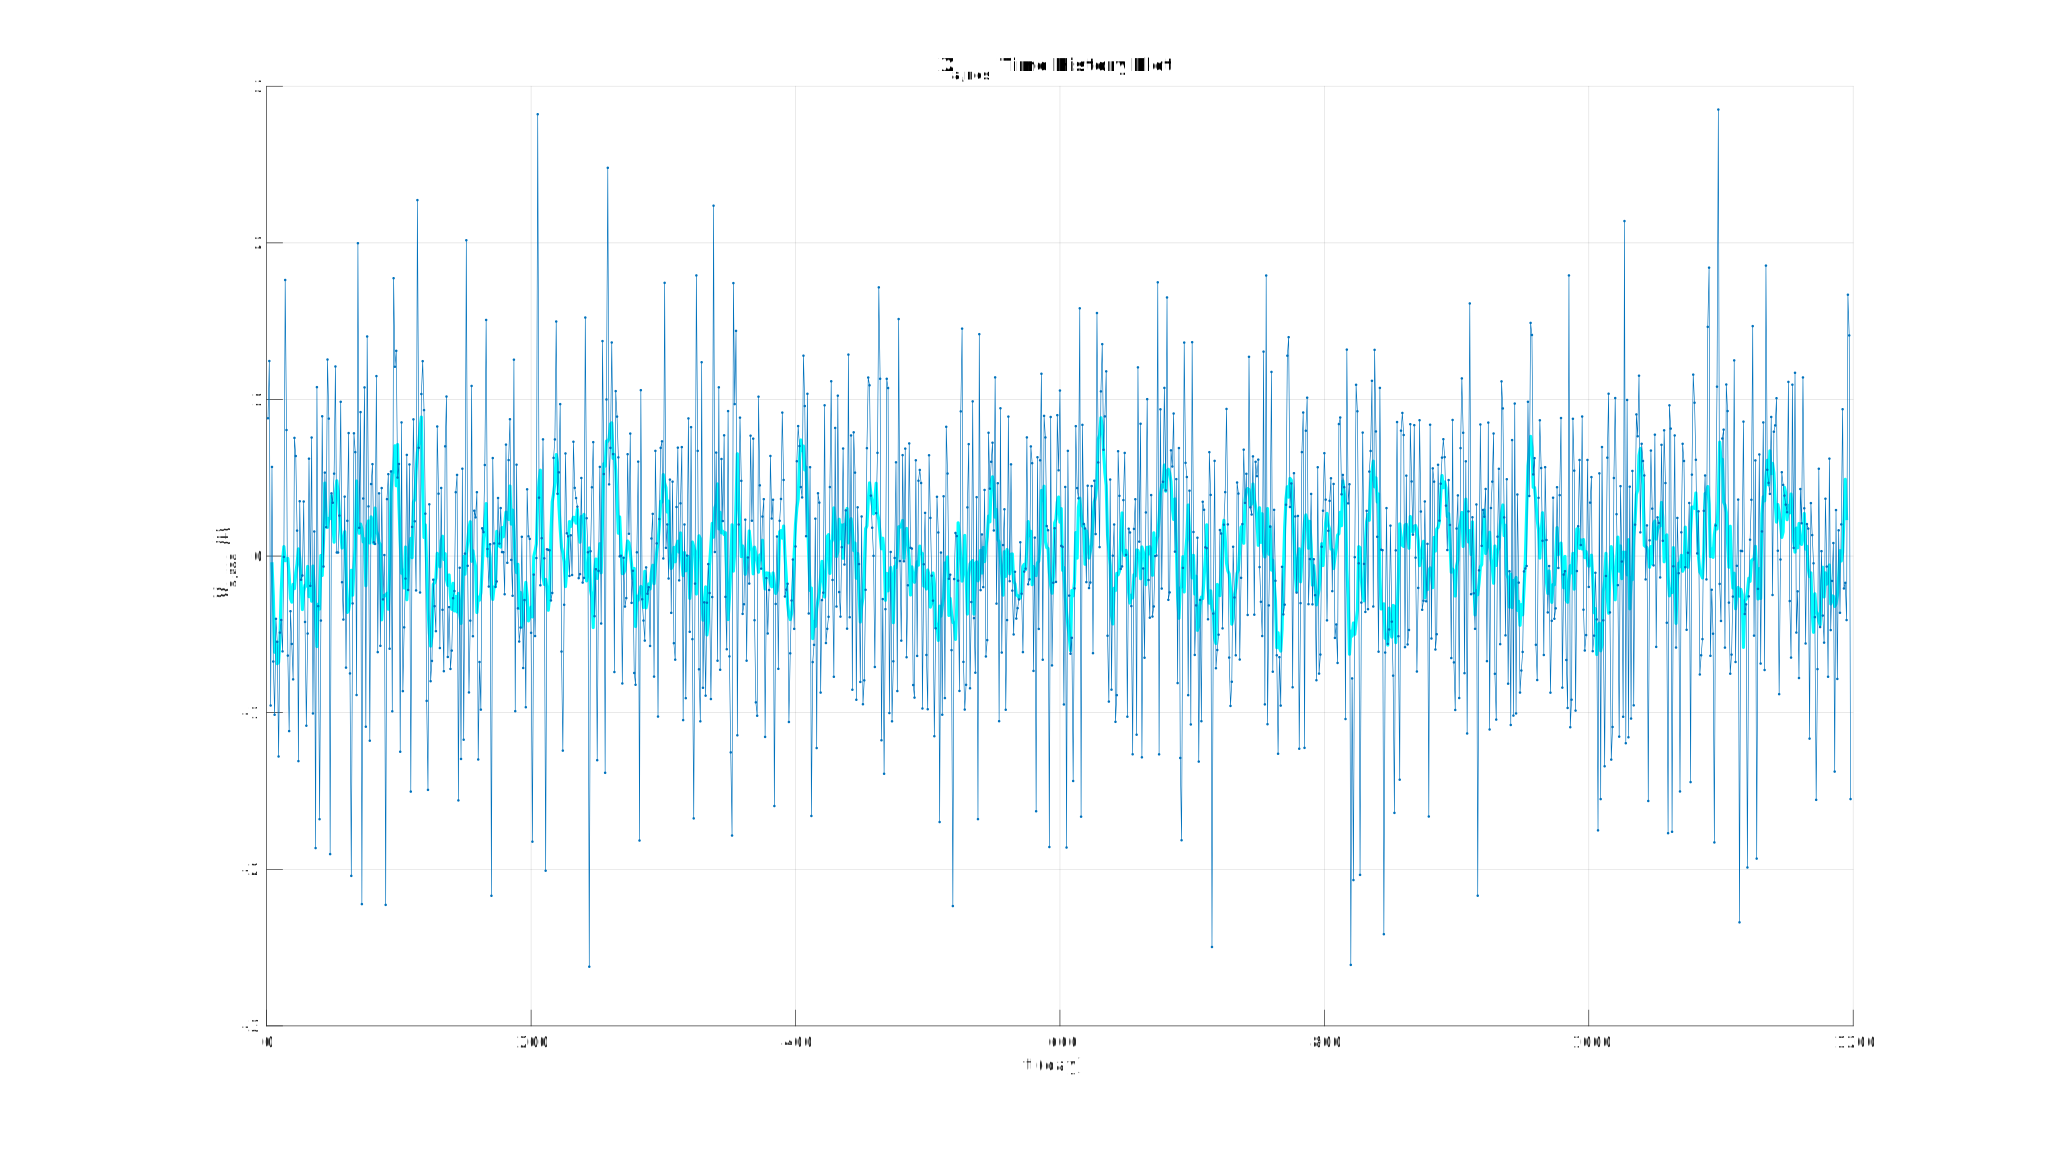
\includegraphics[width=\textwidth]{plots/xa_residuals_history.svg.pdf}
        \caption{Διάγραμμα ιστορίας της χρονοσειράς των υπολοίπων της προσαρμογής του μοντέλου της σχέσης (\ref{eq:xa_model}), $\{X_{a,res}(t) = \hat{z}(t)\}$}
        \label{fig:xa_residuals_history}
    \end{center}
\end{figure}

Στη συνέχεια δίνονται τα διαγράμματα δειγματικής αυτοσυσχέτισης και \tl{p-values} του \tl{Ljung \& Box test} για μέγιστη υστέρηση $\tau$ από 1 έως 30:

\begin{figure}[H]
    \begin{center}
        \includegraphics[width=\textwidth]{plots/xa_residuals_autocorrelation.svg.pdf}
        \caption{Διάγραμμα δειγματικής αυτοσυσχέτισης της σειράς των υπολοίπων της προσαρμογής του μοντέλου της σχέσης (\ref{eq:xa_model}), $r_{\hat{z}_a}(\tau)$}
        \label{fig:xa_residuals_autocorrelation}
    \end{center}
\end{figure}

\begin{figure}[H]
    \begin{center}
        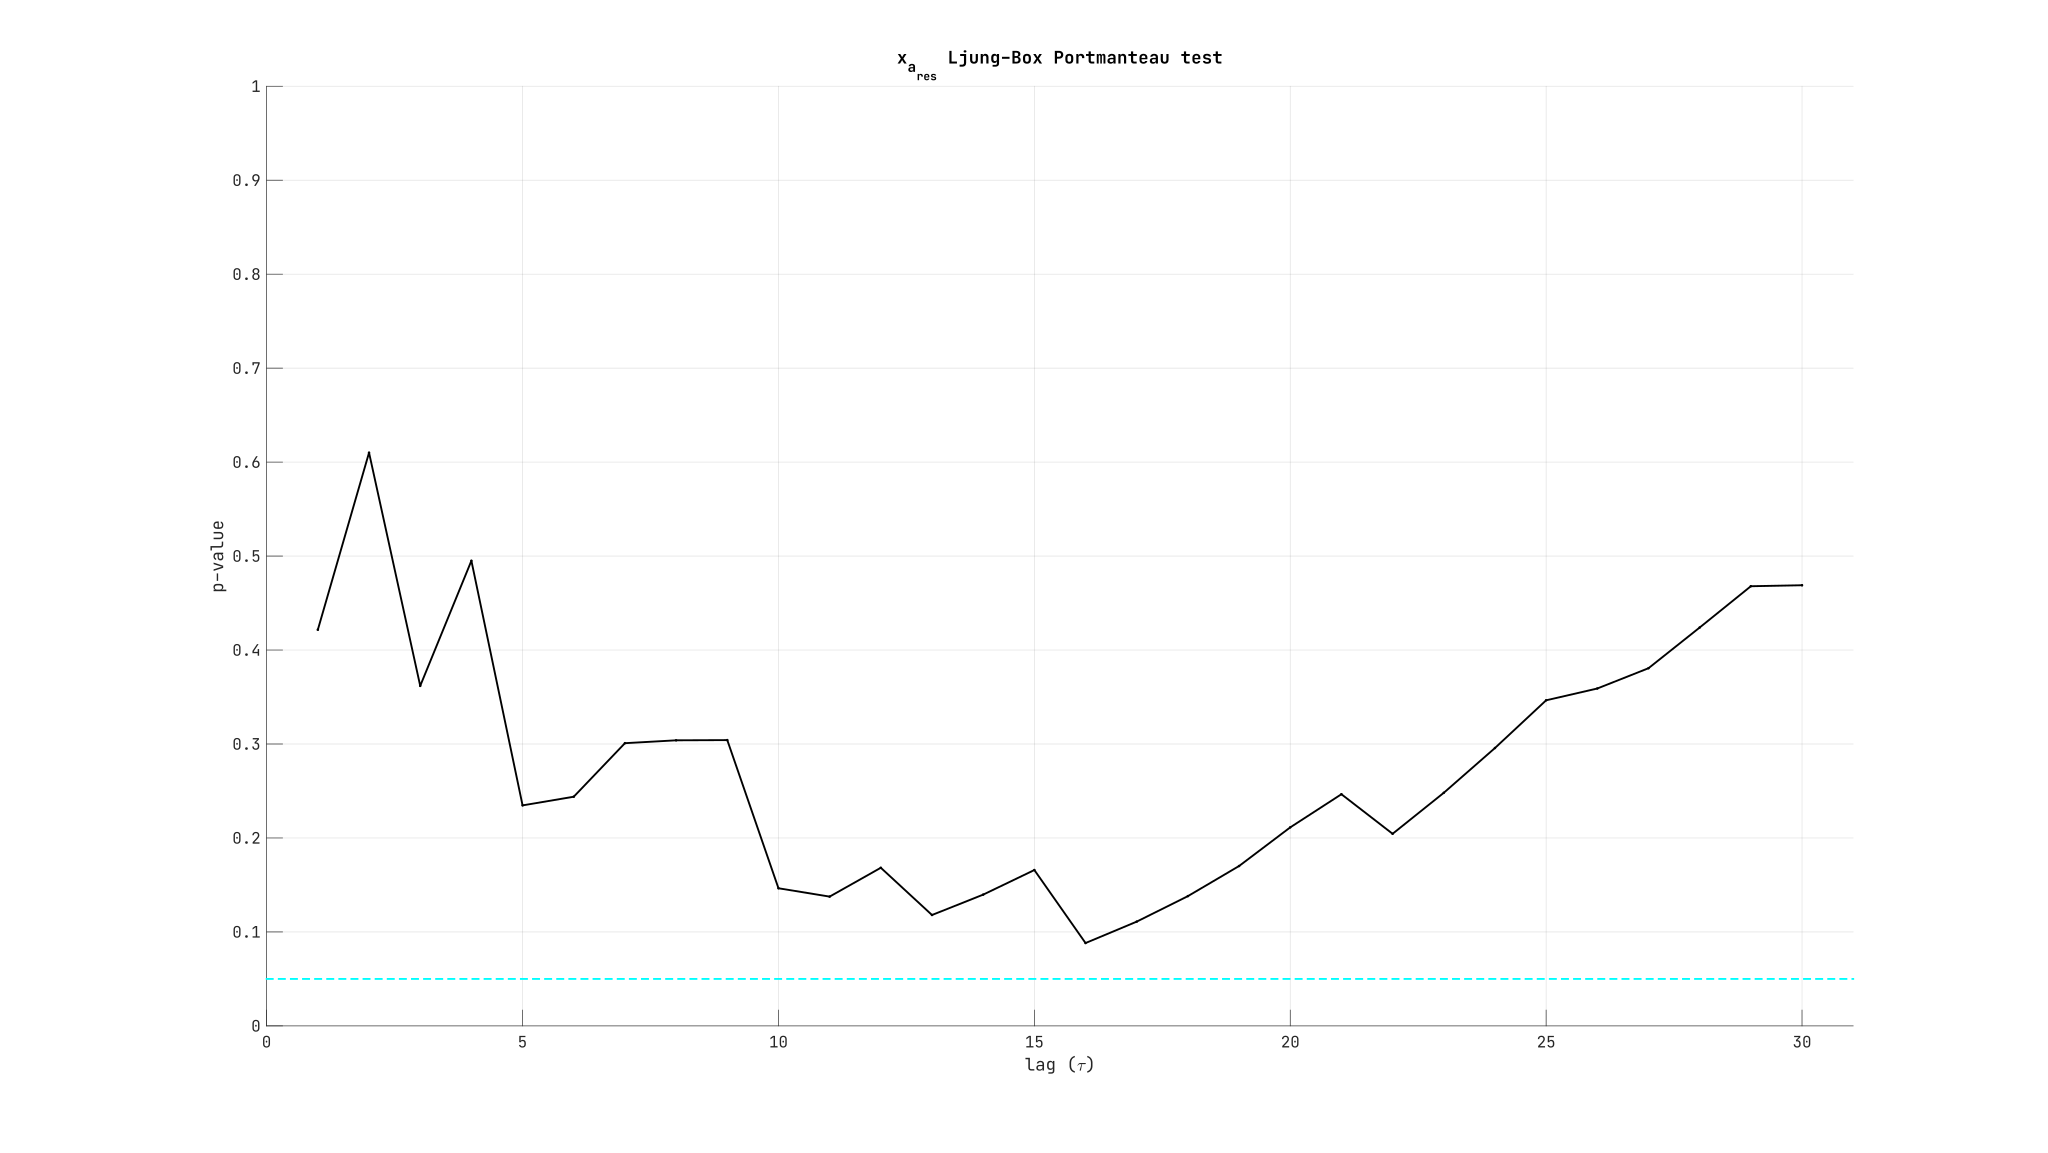
\includegraphics[width=\textwidth]{plots/xa_residuals_portmanteau.svg.pdf}
        \caption{Διάγραμμα των \tl{p-values} του στατιστικόυ ελέγχου ανεξαρτησίας \tl{Portmanteau (Ljung \& Box test)} των υπολοίπων της προσαρμογής του μοντέλου της σχέσης (\ref{eq:xa_model}). Σημειώνεται με διακεκομμένη γραμμή το όριο απόφασης όπου όπως φαίνεται η μηδενική υπόθεση $H_0$ (η σειρά των υπολοίπων είναι \tl{iid}) δεν απόρριπτεται για καμία από τις 30 υστερήσεις.}
        \label{fig:xa_residuals_portmanteau}
    \end{center}
\end{figure}

Αμφότερα τα σχήματα \ref{fig:xa_residuals_autocorrelation} και \ref{fig:xa_residuals_portmanteau} παραπάνω φανερώνουν ότι η προσαρμογή του $MA(1)$ μοντέλου της σχέσης (\ref{eq:xa_model}) είναι επιτυχής αφού αφήνει ασυσχέτιστα υπόλοιπα. Αυτό φαίνεται στο διάγραμμα αυτοσυσχετίσεων των υπολοίπων όπου μόνο για υστέρηση 10 η αυτοσυσχέτιση μόλις που ξεπερνάει το όριο σημαντικότητας (κάτι που επιτρέπεται από το επίπεδο εμπιστοσύνης) ενώ όλες οι υπόλοιπες αυτοσυσχετίσεις είναι στατιστικά μηδενικές. Αντίστοιχα αποτελέσμστα λαμβάνουμε και από τον έλεγχο ανεξαρτησίας \tl{Portmanteau} όπου η μηδενική υπόθεση πως η σειρά των υπολοίπων είναι \tl{iid} δεν απορρίπτεται για καμία από τις 30 υστερήσεις. Με ασφάλεια μπορούμε να πούμε πως η προσαρμογή αφήνει λευκό θόρυβο ως σειρά υπολοίπων.

\par Τέλος, για λόγους πληρότητας παρεθέτουμε το \tl{NRMSE} των σφαλμάτων προσαρμογής
για πρόβλεψη ενός βήματος μπροστά καθώς και τις ίδιες τις προβλέψεις μαζί με την αρχική χρονοσειρά προβολών του βίντεο \tl{A} με βάση την σχέση (\ref{eq:ya_model}), παρακάτω:

\begin{align}
NRMSE(\hat{X_a}, X_a) = 0.7567
\end{align}

\begin{figure}[H]
    \begin{center}
        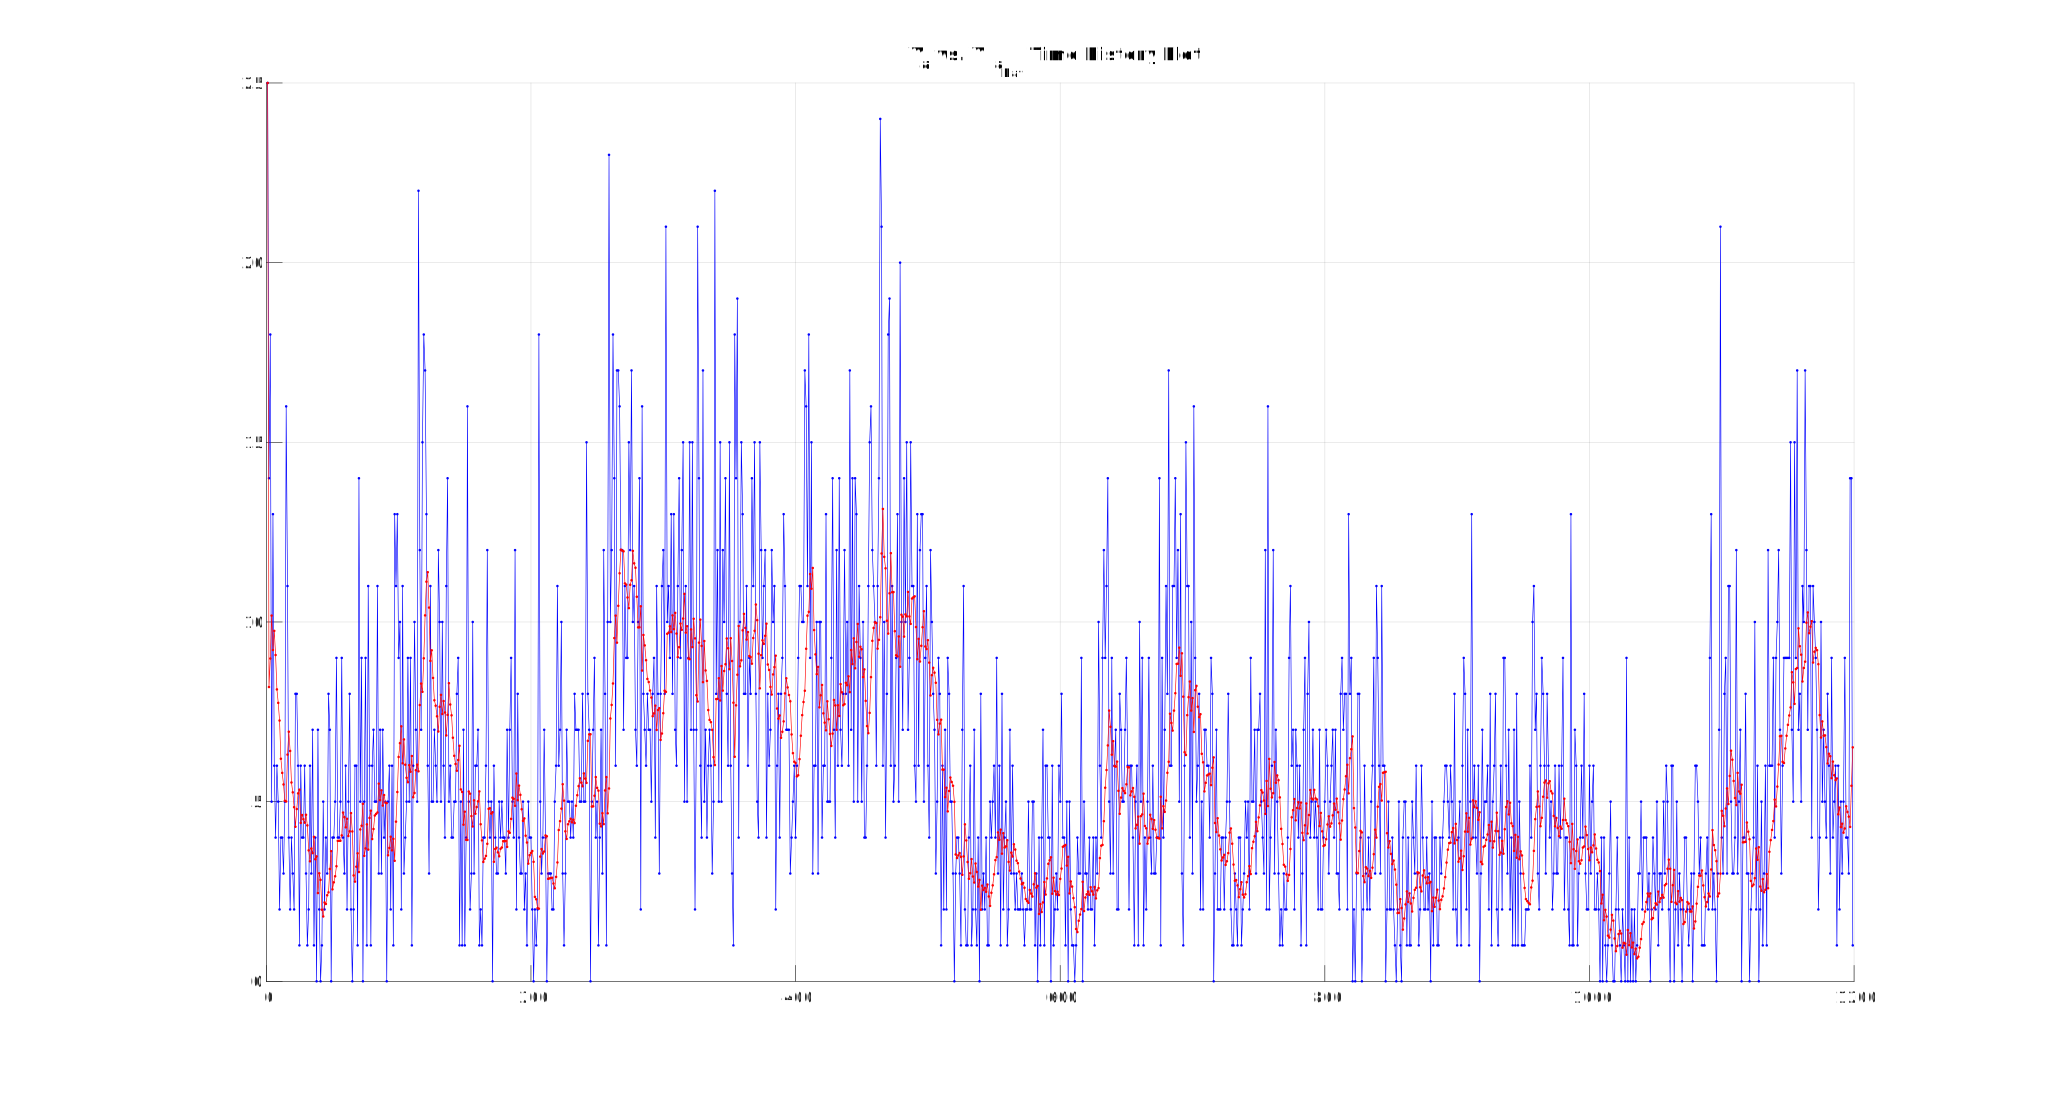
\includegraphics[width=\textwidth]{plots/ya_vs_ya_hat_history.svg.pdf}
        \caption{Διάγραμμα ιστορίας της αρχικής χρονοσειράς προβολών του βίντεο (μπλε) \tl{A} καθώς και τις προβλέψεις ενός βήματος μπροστά αυτής με βάση το προσαρμοσμένο μοντέλο $MA(1)$ και τη σχέση (\ref{eq:ya_model}) (κόκκινο).}
        \label{fig:ya_vs_ya_hat_history}
    \end{center}
\end{figure}